\section{Koncepcja mobilnej stacji naziemnej}

Zgodnie z planem projektu powstała stacja składająca się z:

\begin{itemize}
 \item dwu-częściowego rotora wraz ze sterownikiem, czujnikami położenia i kompasem,
 \item wykorzystanego radia programowalnego SDR z oprogramowaniem do dekodowania odbieranego sygnału,
 \item układu FPGA z możliwością realizacji własnego demodulatora na innym paśmie,
 \item układu zasilania składającego się z: 
    \begin{itemize}
    \item akumulatora samochodowego o pojemności 20Ah i napięciu 12 V,
    \item przetwornicy do napięcia 5V do zasilenia układów logicznych rotora,
    \item prostownikia do ładowania akumulatora,
    \item przetwornicy do napięcia zmiennego 230V ze standardowym gniazdkiem do zasilania ewentualnych peryferiów takich jak laptop,
    \end{itemize}
\end{itemize}

Ponieważ nie mamy wykształcenia w zakresie wykonywania konstrukcji mechanicznych to nasz projekt jest realizacją wysoce amatorską, ale funkcjonalną. Największym wyzwaniem był dobór odpowiednich przekładni do uzyskania precyzyjnych (wolnych) obrotów i dużego momentu siły.

Schemat ideowy działania całej stacji przedstawiono na rysunku \ref{stacschem}.

\begin{figure}[!htbp]
    \centering
    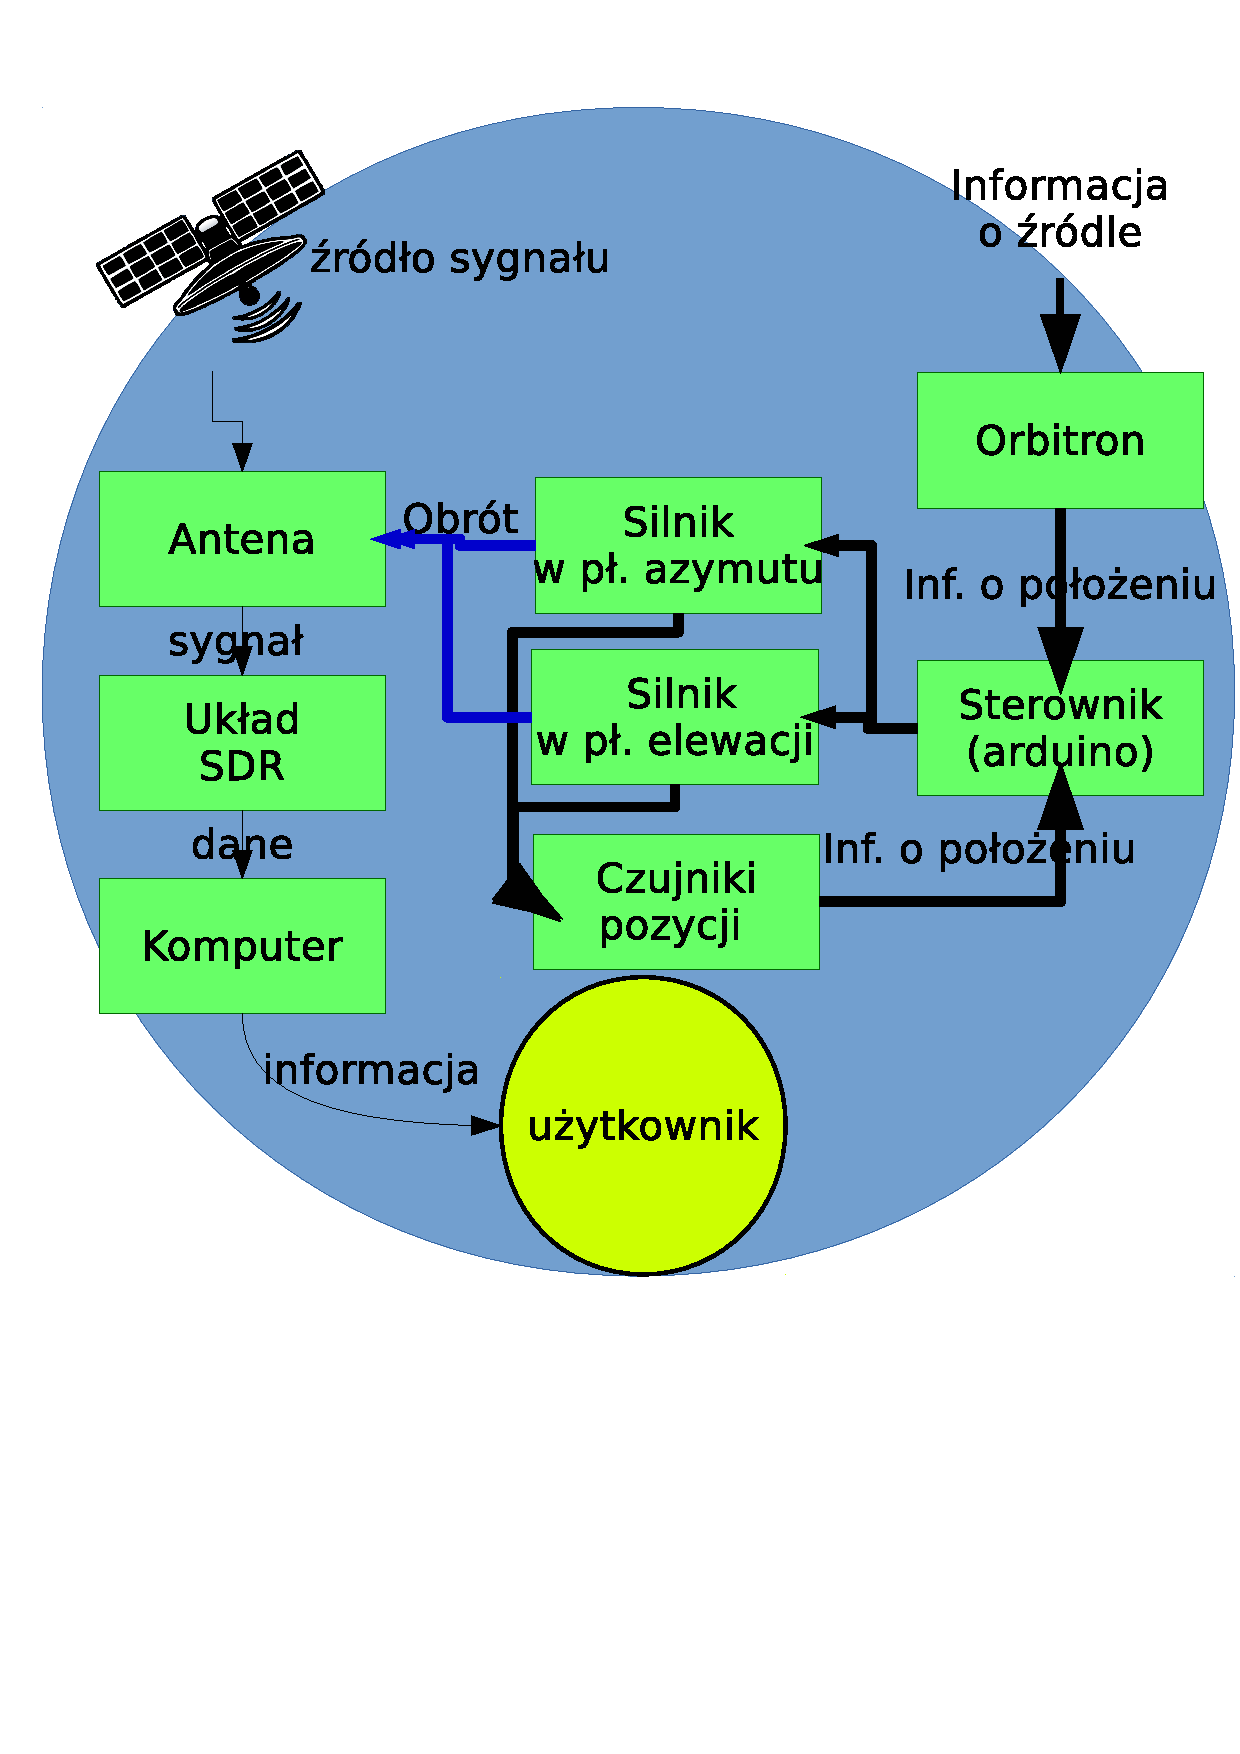
\includegraphics[width=0.7\textwidth]{schemat_skik2017}
    \caption{Schemat blokowy systemu stacji naziemnej}
    \label{stacschem}
\end{figure}
